\documentclass{article}

\usepackage{graphicx}
\usepackage{blindtext}
\usepackage{wrapfig}

\author{Javier Portillo}
\title{The Logic of Images and Figure in {\LaTeX}}

\begin{document}

\maketitle

\begin{center}
	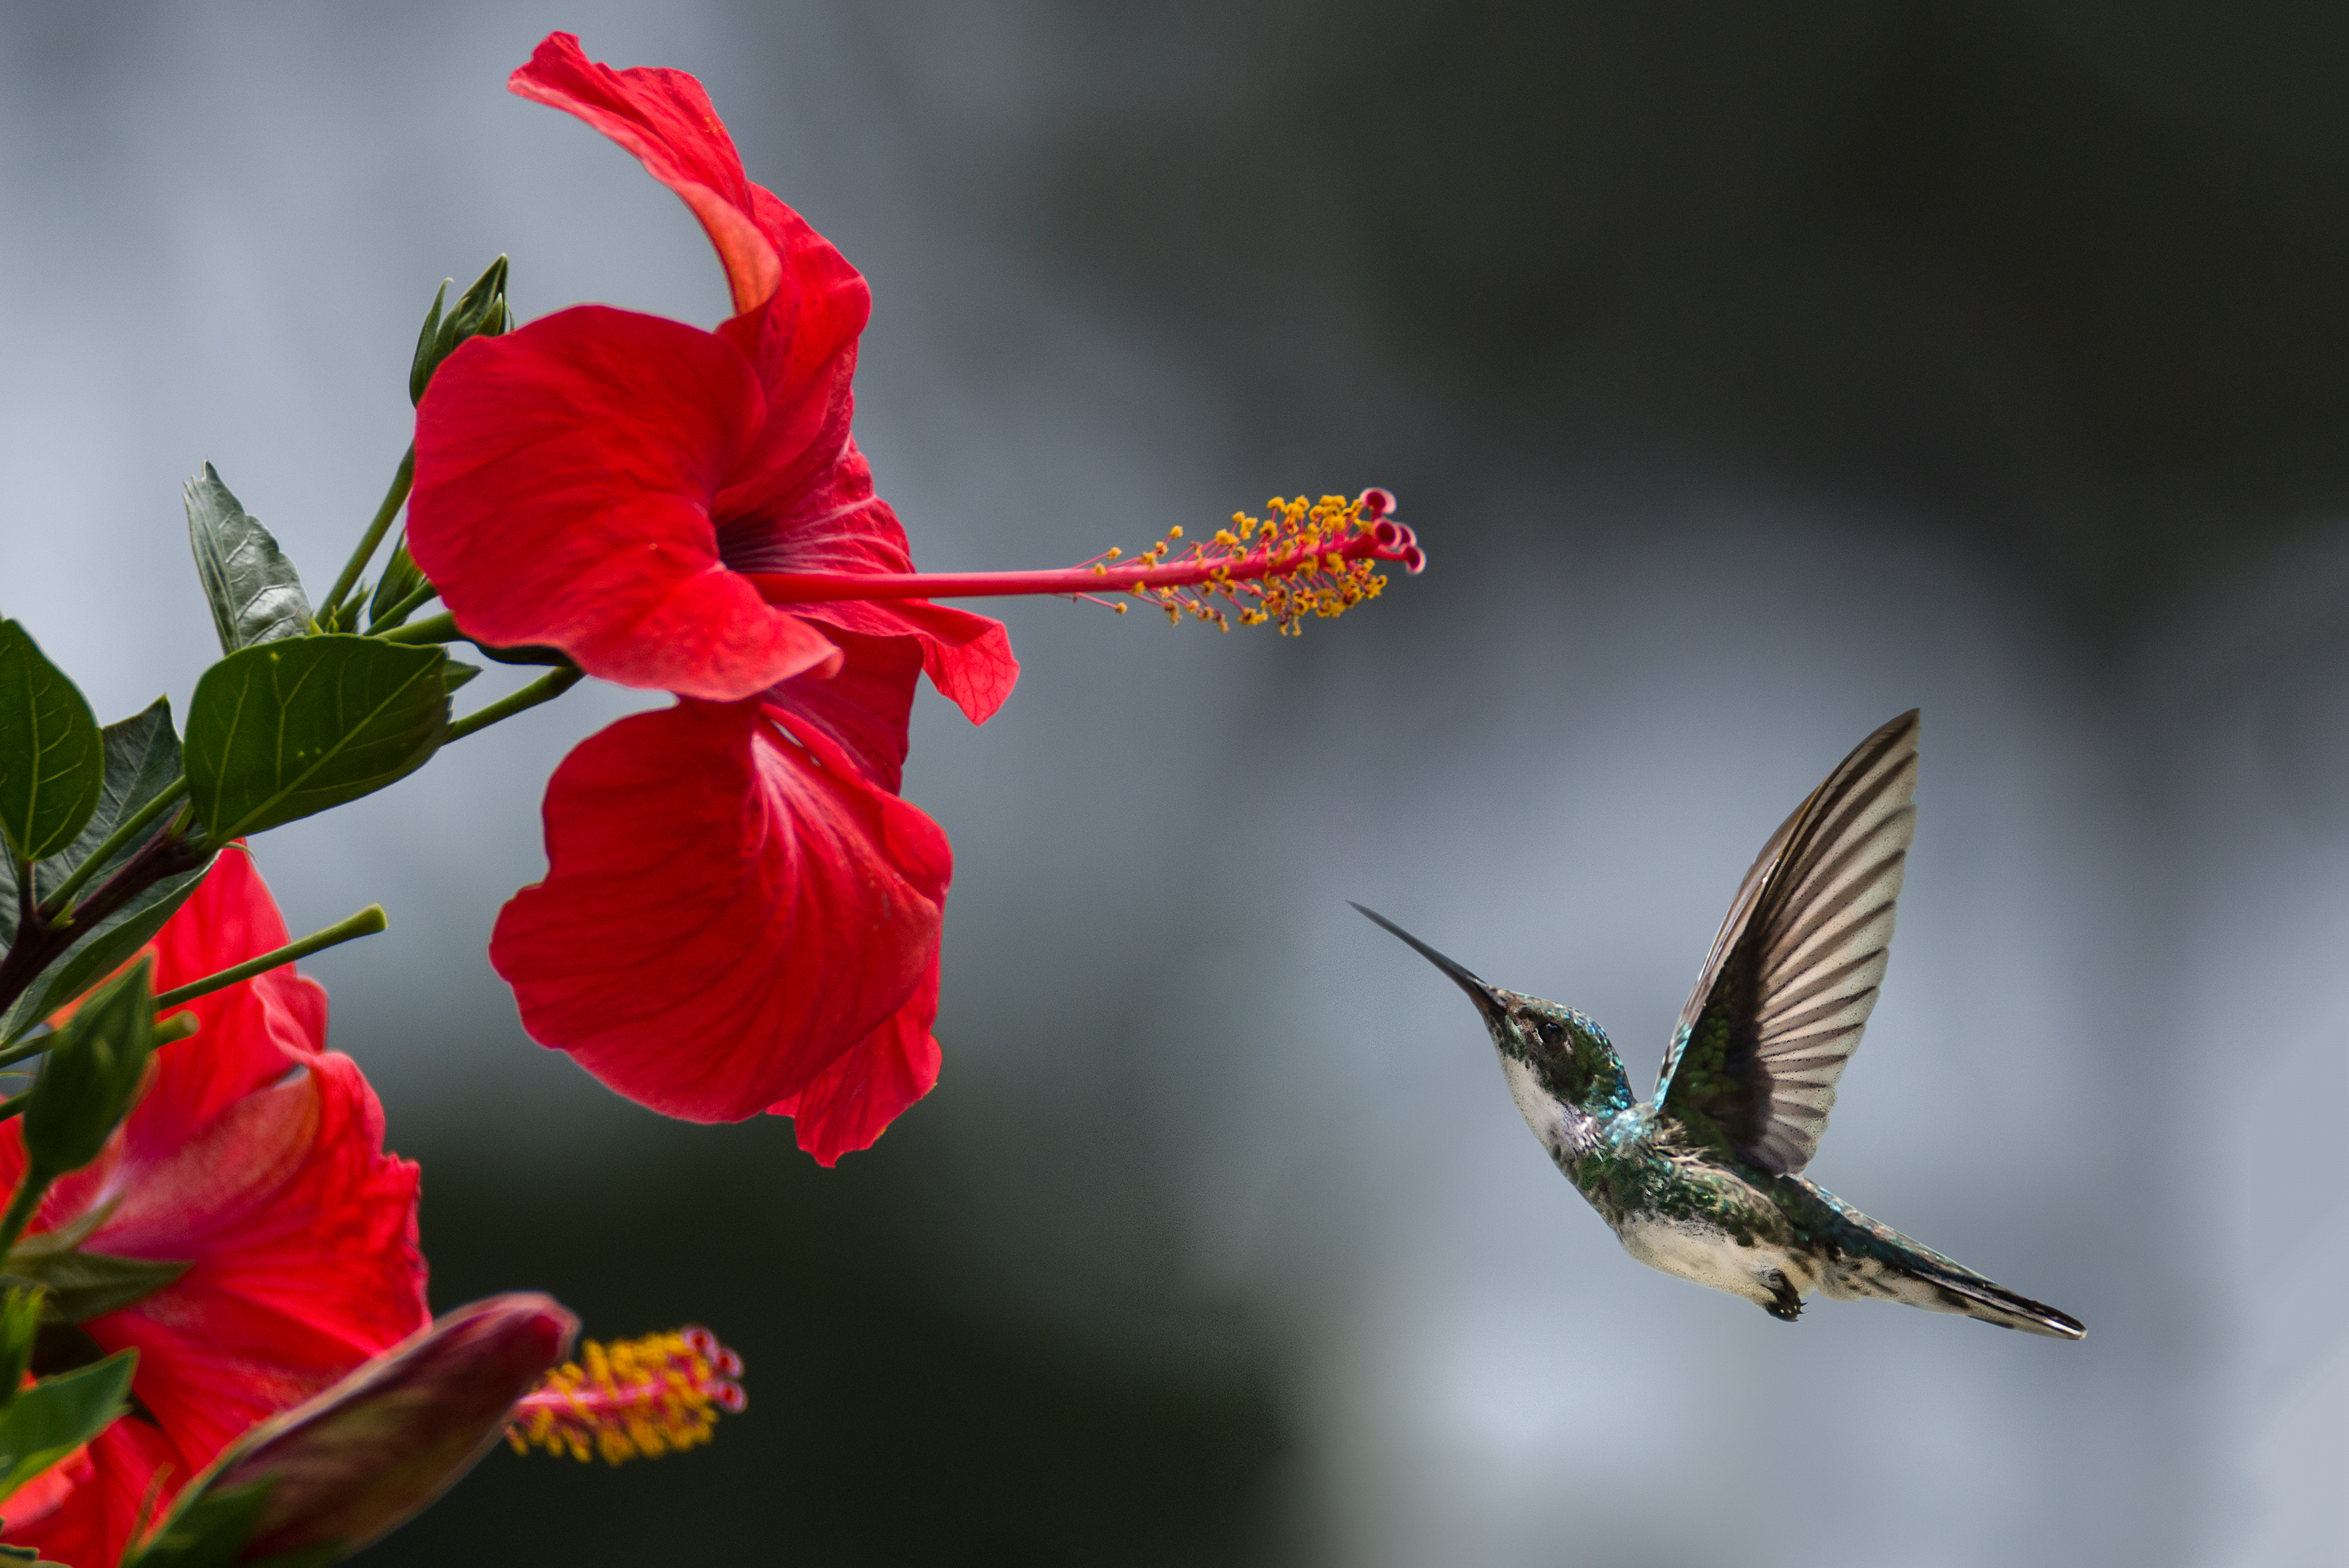
\includegraphics[width=0.7\textwidth]{picture.jpeg}
\end{center}

\blindtext

\blindtext

In the figure below, you can see a pretty birb.

\begin{figure}[h]
  \centering
  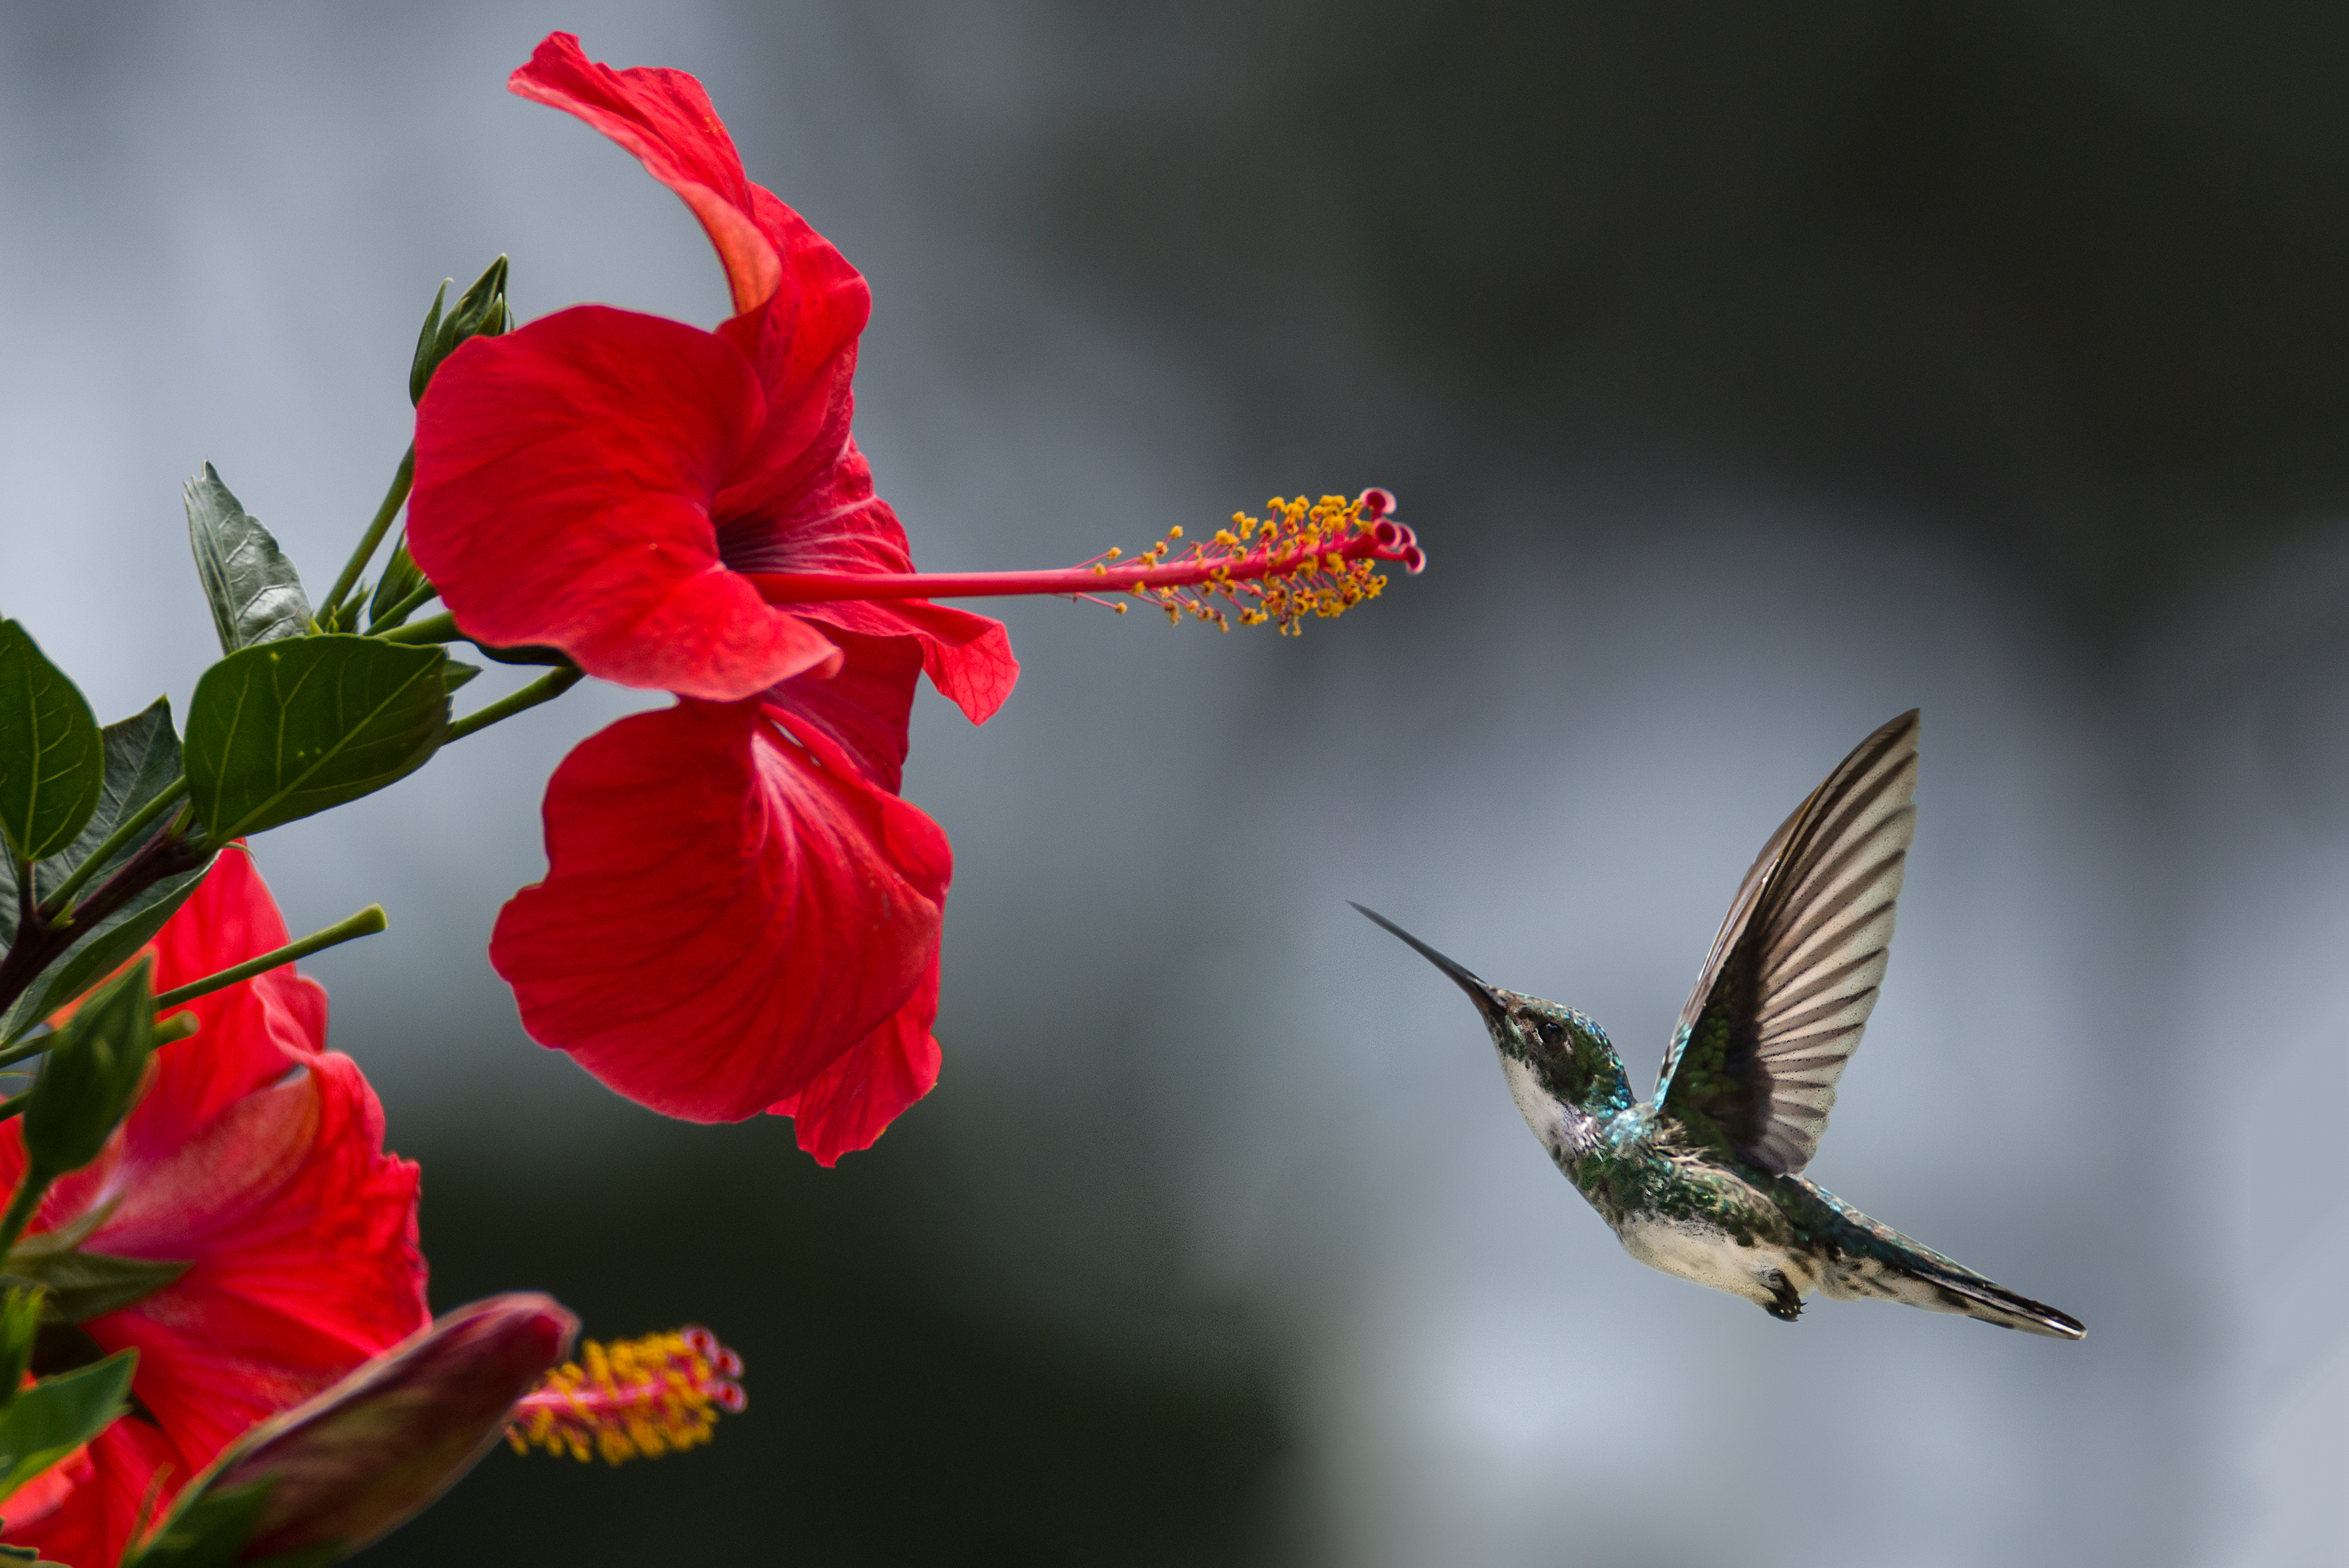
\includegraphics[width=0.7\textwidth]{picture.jpeg}
  \caption{A birb}
\end{figure}

\blindtext
\blindtext
\blindtext

\begin{wrapfigure}{r}{3in}
  \centering
	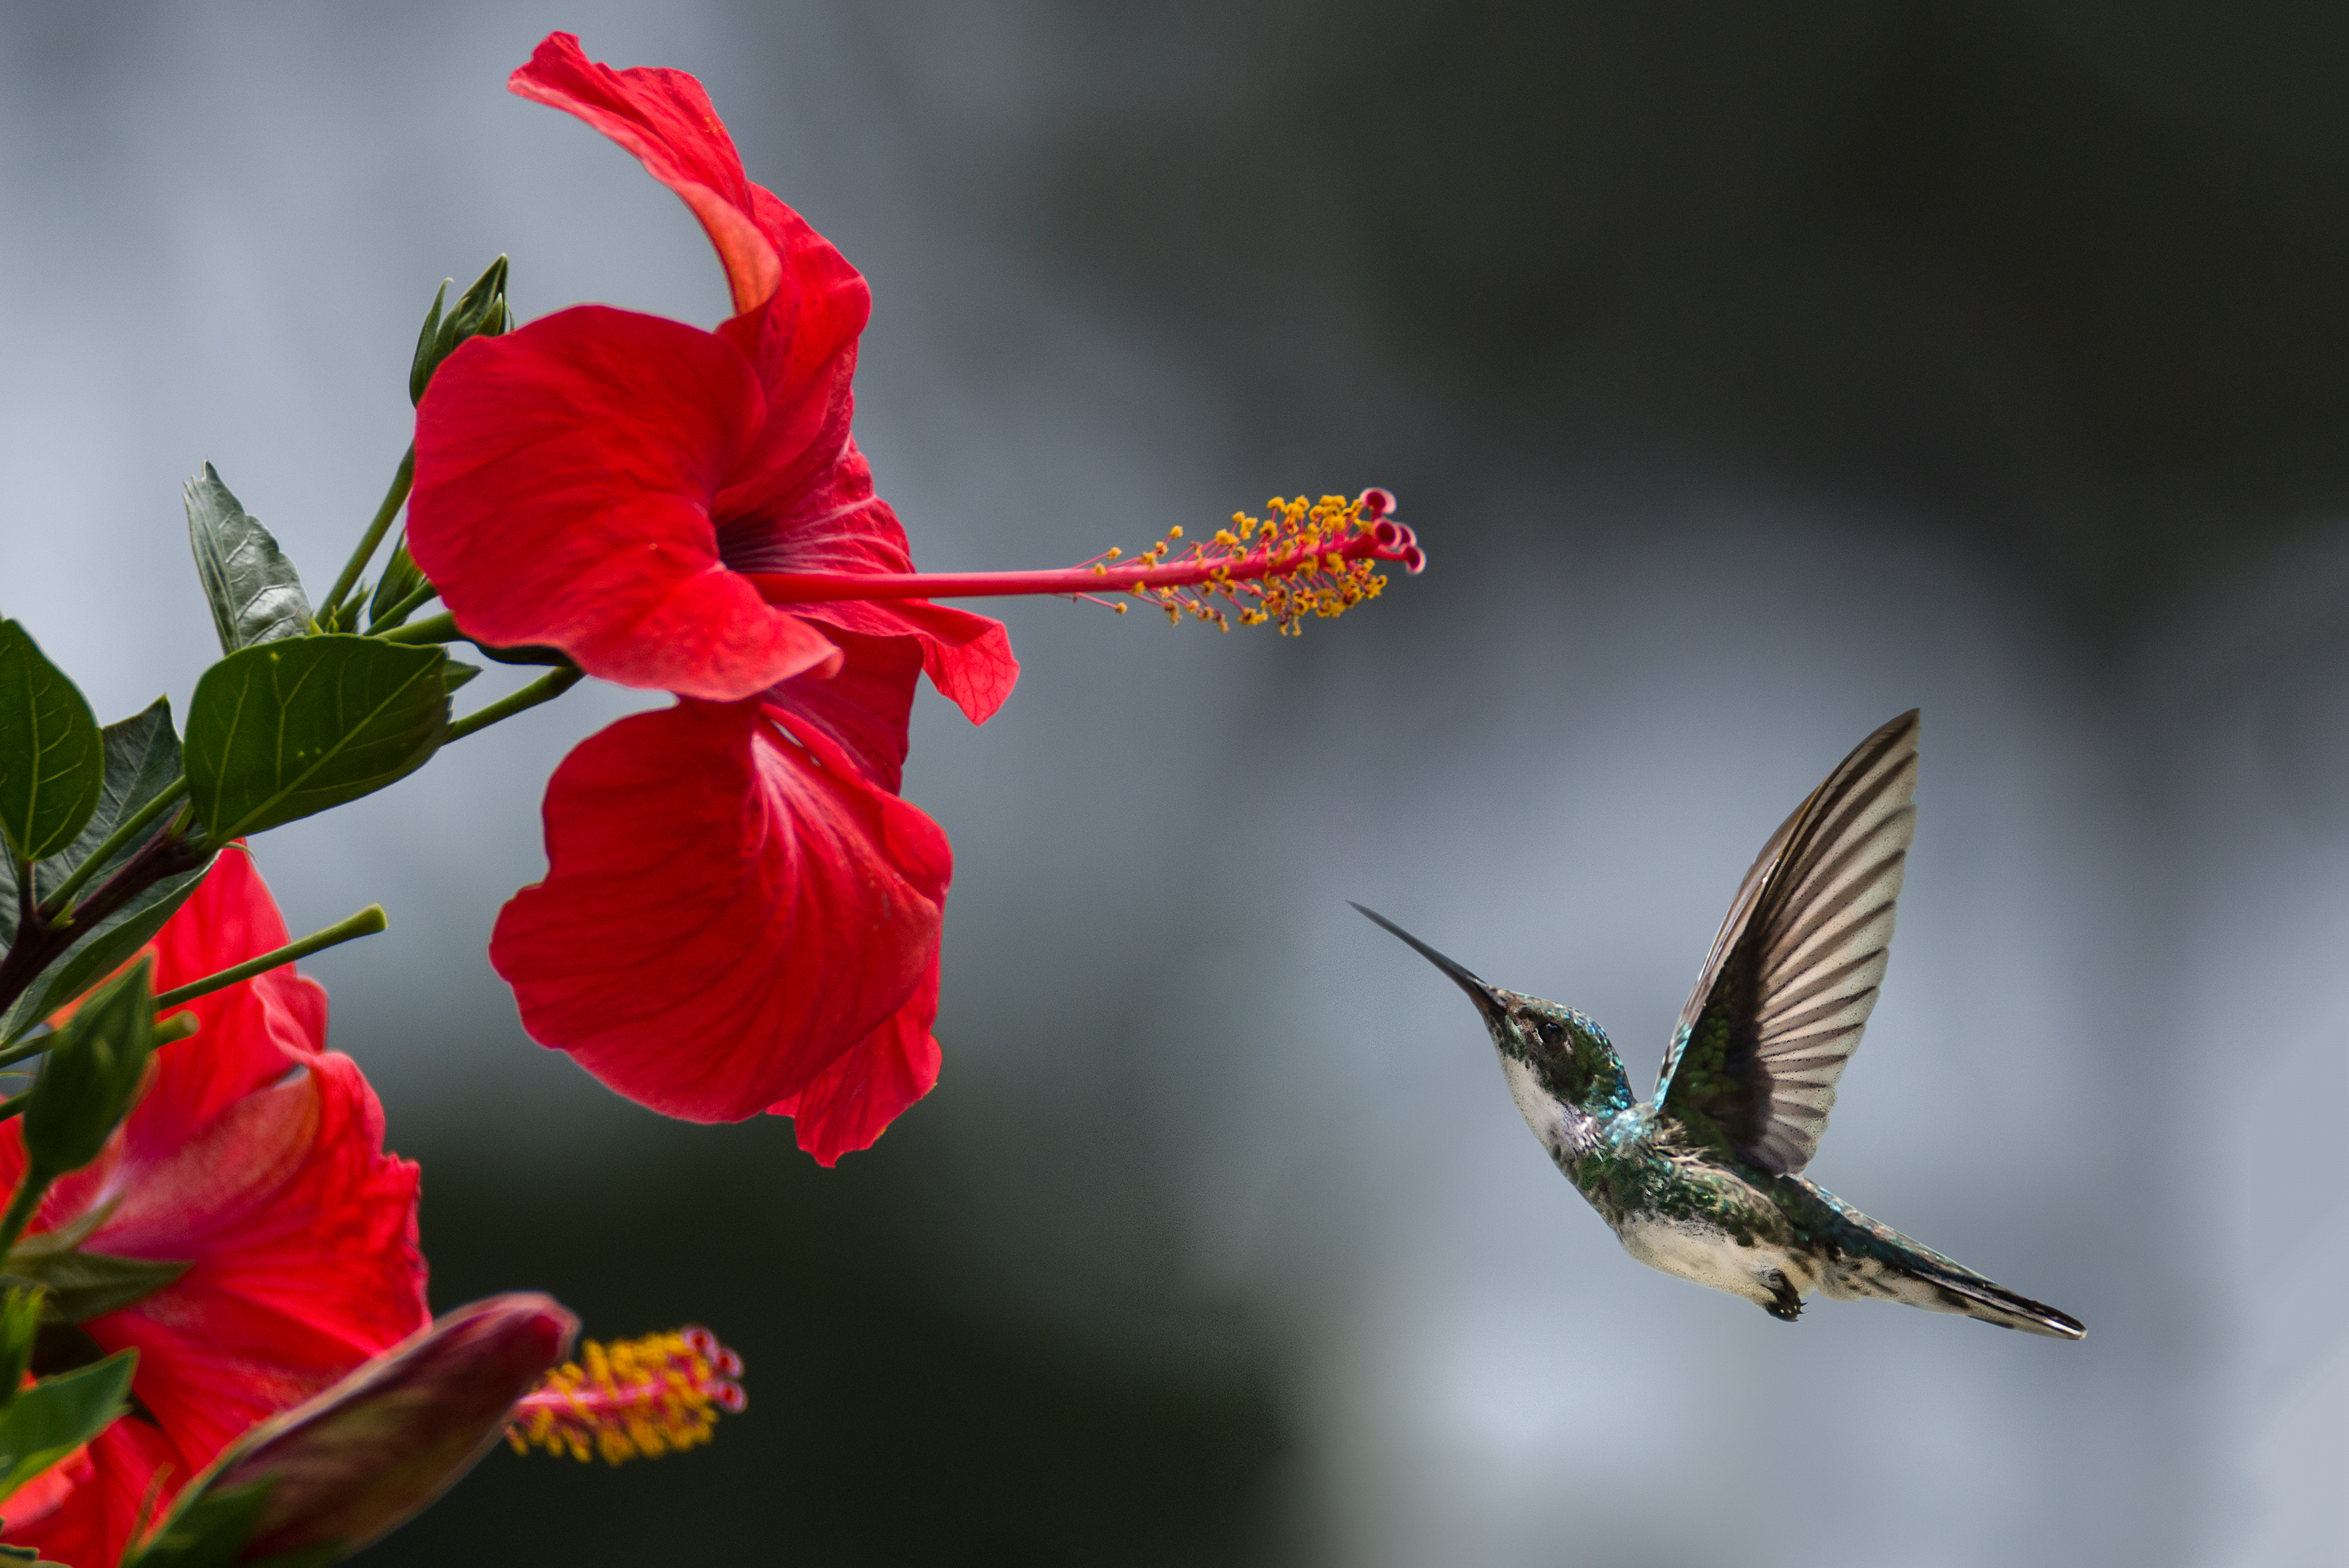
\includegraphics[width=2.5in]{picture.jpeg}
  \caption{another same birb}
  \label{birbpic}
\end{wrapfigure}

Please refer to Figure \ref{birbpic}.

\blindtext
\blindtext

\end{document}
